\documentclass[a4paper,11pt]{article}

\usepackage[T1]{fontenc}
\usepackage[utf8]{inputenc}
\usepackage{graphicx}
\usepackage{xcolor}

\renewcommand\familydefault{\sfdefault}
\usepackage{tgheros}

\usepackage{amsmath,amssymb,amsthm,textcomp}
\usepackage{enumerate}
\usepackage{multicol}
\usepackage{tikz}
\usepackage{pdfpages}


\graphicspath{ {.} }
\usepackage{geometry}
\geometry{left=25mm,right=25mm,%
bindingoffset=0mm, top=20mm,bottom=20mm}



\usepackage{tabularx,lipsum,environ,amsmath,amssymb}

\makeatletter
\newcommand{\problemtitle}[1]{\gdef\@problemtitle{#1}}% Store problem title
\newcommand{\problemquestion}[1]{\gdef\@problemquestion{#1}}% Store problem question
\newcommand{\problemsolution}[1]{\gdef\@problemsolution{#1}}% Store problem input
\NewEnviron{problem}{
  \problemtitle{}\problemquestion{}\problemsolution{}% Default input is empty
  \BODY% Parse input
  \par\addvspace{.5\baselineskip}
  \noindent
  \begin{tabularx}{\textwidth}{@{\hspace{\parindent}} l X c}
    \multicolumn{2}{@{\hspace{\parindent}}l}{\@problemtitle} \\% Title
    \textbf{Description:} & \@problemquestion \\% Question
        \textbf{Solution:} & \@problemsolution % Input
  \end{tabularx}
  \par\addvspace{.5\baselineskip}
}
\makeatother







\linespread{1.3}

\newcommand{\linia}{\rule{\linewidth}{0.5pt}}

% custom theorems if needed
\newtheoremstyle{mytheor}
    {1ex}{1ex}{\normalfont}{0pt}{\scshape}{.}{1ex}
    {{\thmname{#1 }}{\thmnumber{#2}}{\thmnote{ (#3)}}}

\theoremstyle{mytheor}
\newtheorem{defi}{Definition}

% my own titles
\makeatletter
\renewcommand{\maketitle}{
\begin{center}
\vspace{2ex}
{\huge \textsc{\@title}}
\vspace{1ex}
\\
\linia\\
\@author \hspace{100ex} m.plevako@innopolis.university \hspace{100ex} BS18-02 \hspace{100ex} Variant (c)

\vspace{4ex}
\end{center}
}
\makeatother
%%%

% custom footers and headers
\usepackage{fancyhdr}
\pagestyle{fancy}
\lhead{}
\chead{}
\rhead{}
\lfoot{Assignment \textnumero{} 2}
\cfoot{}
\rfoot{Page \thepage}
\renewcommand{\headrulewidth}{0pt}
\renewcommand{\footrulewidth}{0pt}
%

% code listing settings
\usepackage{listings}
\lstset{
    language=Python,
    basicstyle=\ttfamily\small,
    aboveskip={1.0\baselineskip},
    belowskip={1.0\baselineskip},
    columns=fixed,
    extendedchars=true,
    breaklines=true,
    tabsize=4,
    prebreak=\raisebox{0ex}[0ex][0ex]{\ensuremath{\hookleftarrow}},
    frame=lines,
    showtabs=false,
    showspaces=false,
    showstringspaces=false,
    keywordstyle=\color[rgb]{0.627,0.126,0.941},
    commentstyle=\color[rgb]{0.133,0.545,0.133},
    stringstyle=\color[rgb]{01,0,0},
    numbers=left,
    numberstyle=\small,
    stepnumber=1,
    numbersep=10pt,
    captionpos=t,
    escapeinside={\%*}{*)}
}

%%%----------%%%----------%%%----------%%%----------%%%

\begin{document}

\title{HW \textnumero{} 2}

\author{Matvey Plevako}

\maketitle


\section*{Problem 1}

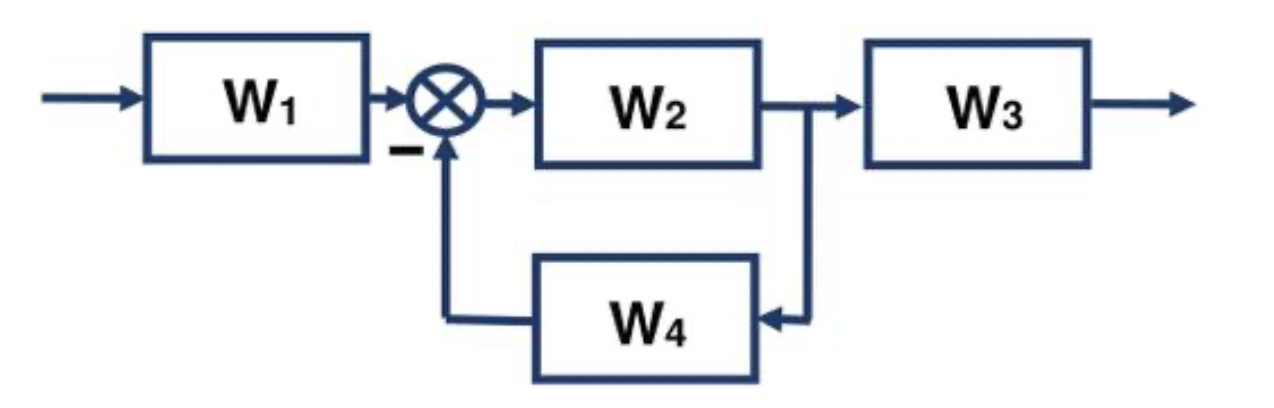
\includegraphics[width=14cm, height=4cm]{1.png}

\begin{problem}
$$W_1 = \frac{2}{s^2 + s - 2}, W_2 = \frac{1}{3s + 2}, W_3 = \frac{s + 1}{s + 0.3}, W_4 = \frac{1}{s + 0.2}$$
  \problemtitle{Part A}
  \problemquestion{Calculate the total Transfer Function of the system.
}
  \problemsolution{
  {\bf Step I}. Reduce negative feedback loop:
  
  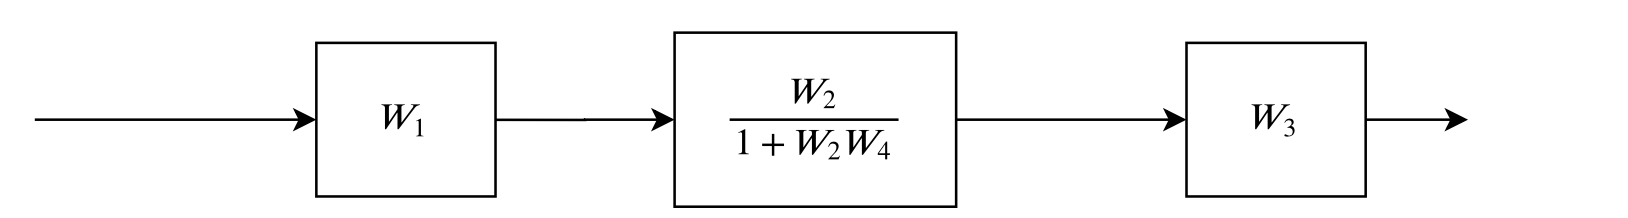
\includegraphics[width=12.5cm, height=2cm]{3.png}
  
  {\bf Step II}. Reduce series connections:
  
  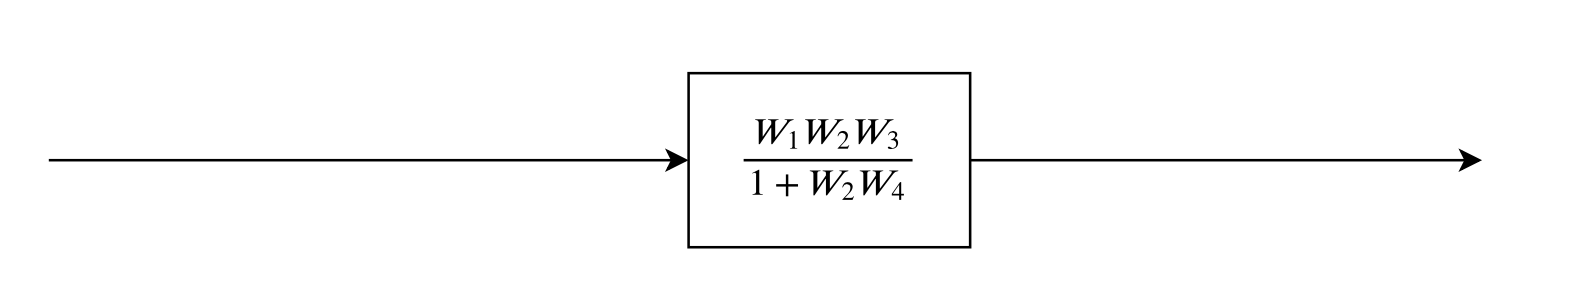
\includegraphics[width=12.5cm, height=2.5cm]{4.png}
  
  {\bf Step III}. Substitute initial functions:
  $$\frac{W_1W_2W_3}{1 + W_2W_4} = \frac{\frac{2}{s^2 + s - 2} * \frac{1}{3s + 2} * \frac{s + 1}{s + 0.3}}{1 + \frac{1}{3s + 2} * \frac{1}{s + 0.2}}$$
  $$\frac{2(s+1)(s+0.2)}{(s+2)(s-1)(s+0.3)((3s+2)(s+0.2) + 1)}$$
  $$Answer: \frac{\frac{2}{3}s^2 + \frac{4}{5}s + \frac{4}{3}}{s^5 + \frac{13}{6}s^4 -\frac{8}{75}s^3 -\frac{22}{15}s^2 -\frac{197}{150}s + \frac{7}{25}}$$

  }
  
  
\end{problem}

\begin{problem}
  \problemtitle{Part B}
  \problemquestion{Build initial system shown in the block diagram and simplified in one Simulink schema and analyze its Step, Impulse and Frequency responses. Results should have a schema with both systems and 3 Scope plots(for each input). Each plot should have 3 lines - input signal, and two outputs from each system.}
  \problemsolution{
  In both plots Frequency and Step, inital TF and the total TF are close to each other. However, on Impulse there is a slight deviation.
  }
\end{problem}
\section*{With Frequency Input}
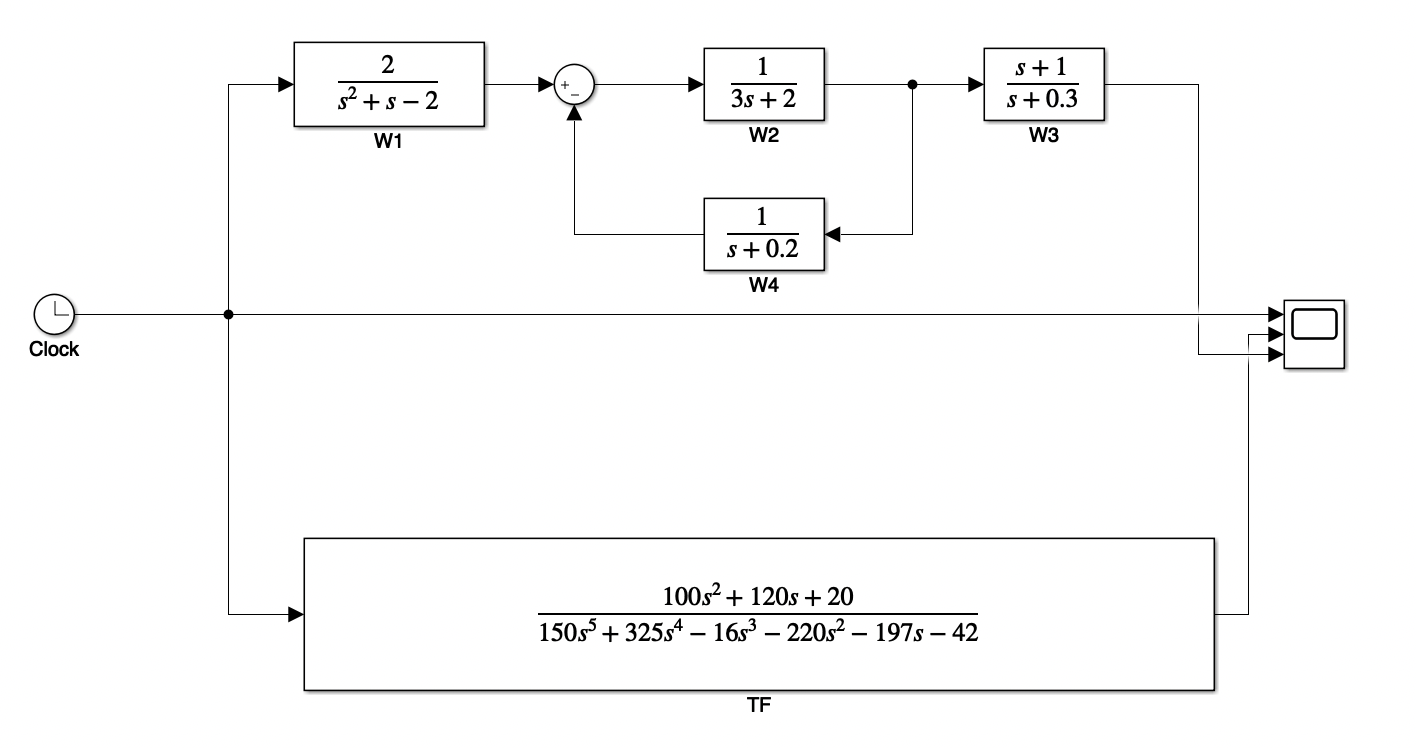
\includegraphics[width=15cm, height=9cm]{clock_1.png}
\section*{Frequency scope}
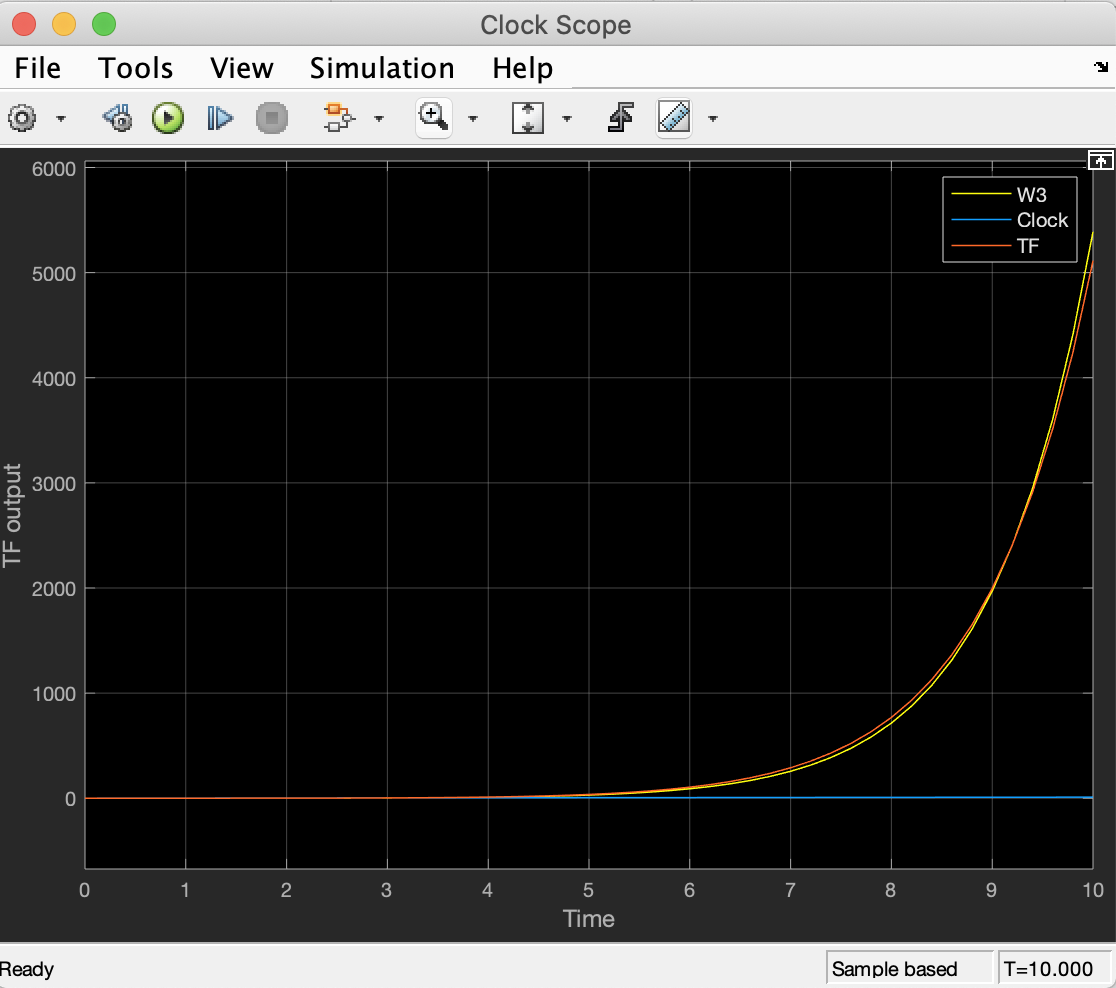
\includegraphics[width=15cm, height=10cm]{clock_2.png}
\section*{With step Input}
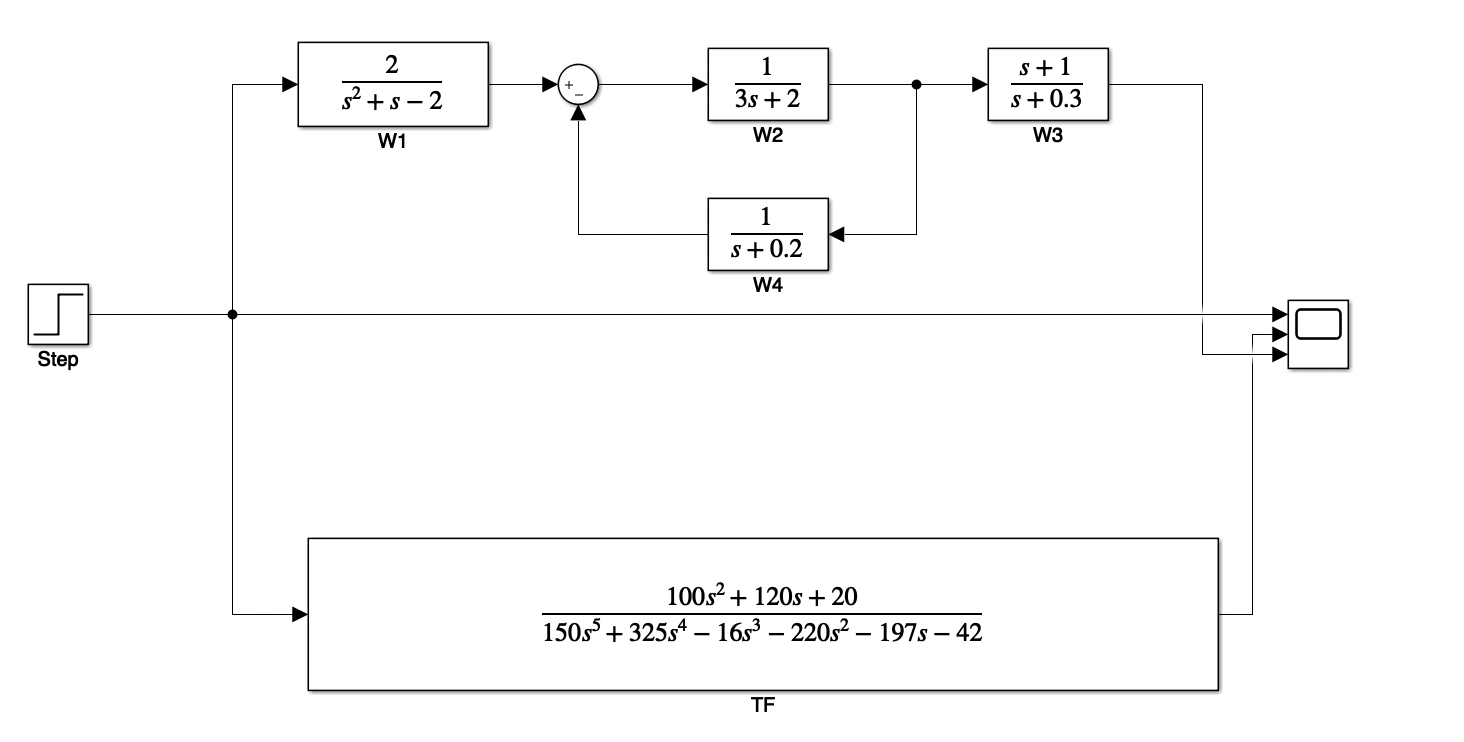
\includegraphics[width=15cm, height=9cm]{step_1.png}
\section*{Step scope}
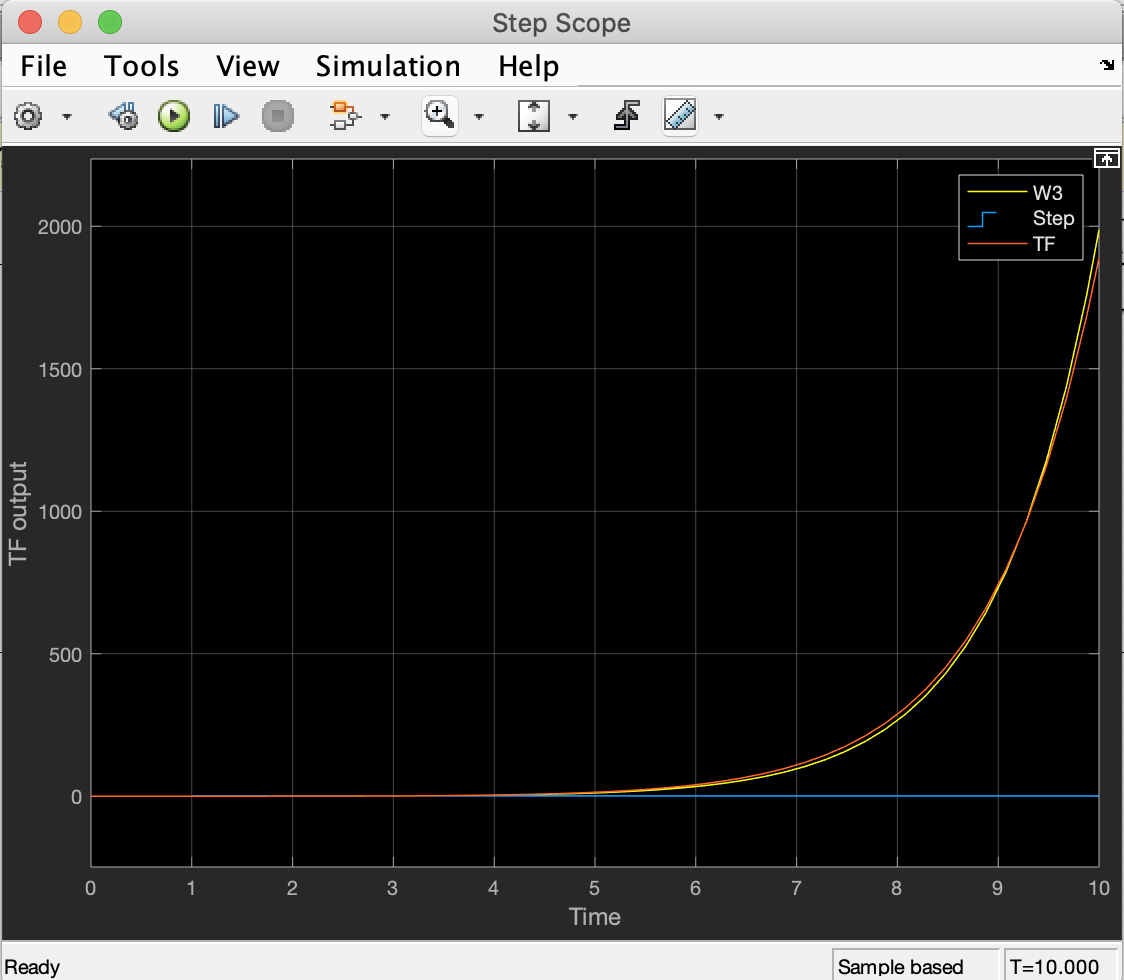
\includegraphics[width=15cm, height=10cm]{step_2.png}
\section*{With Impulse Input}
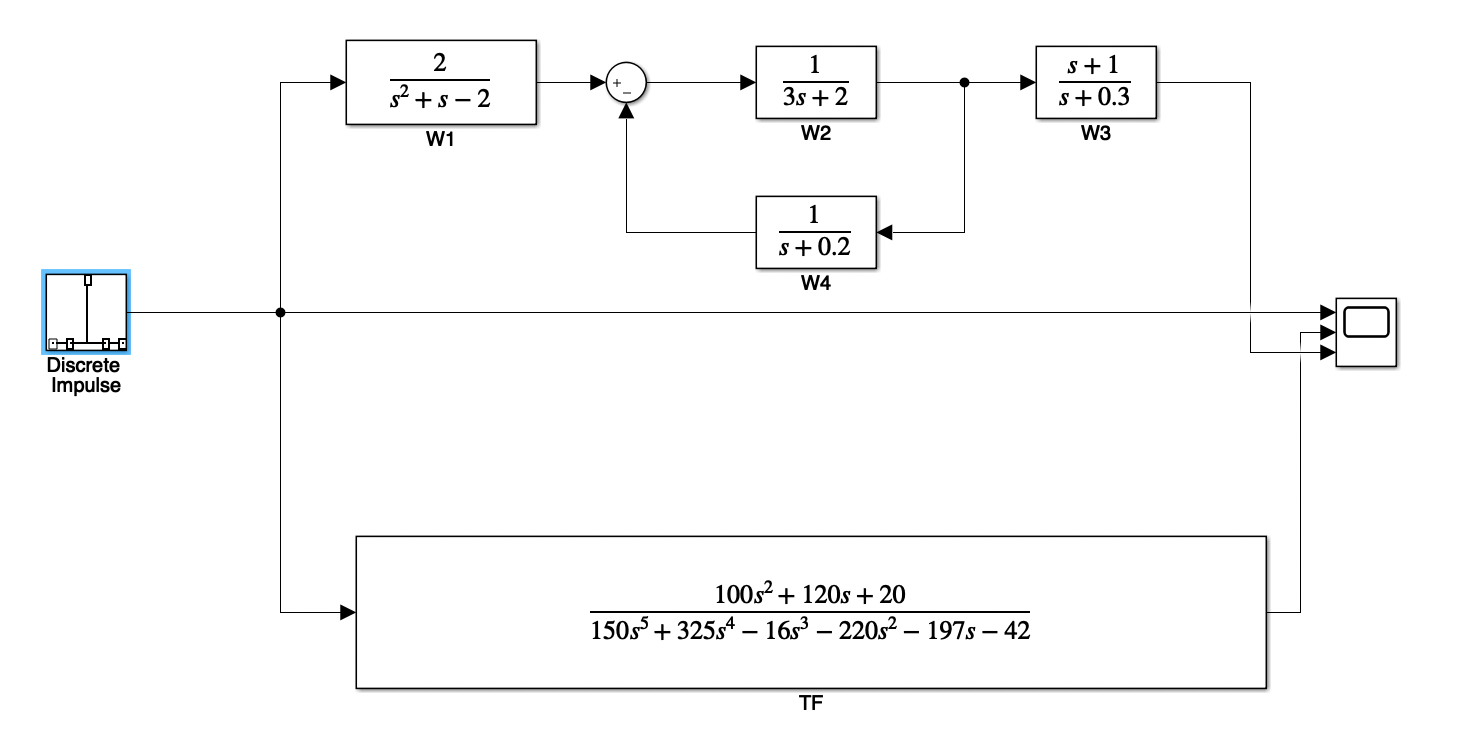
\includegraphics[width=15cm, height=9cm]{impulse_1.png}
\section*{Impulse scope}
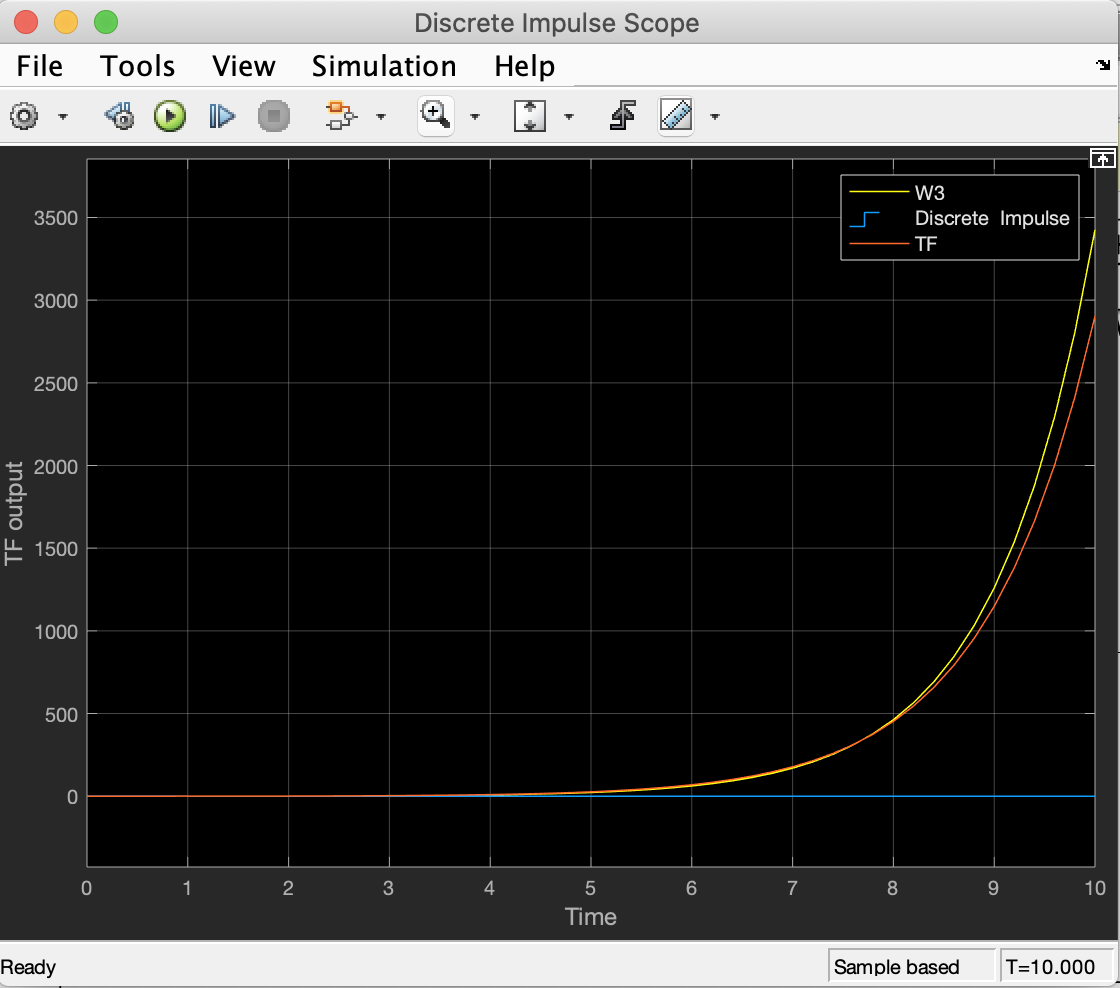
\includegraphics[width=15cm, height=10cm]{impulse_2.png}


\begin{problem}
  \problemtitle{Part C}
  \problemquestion{For one of the inputs (write down what you choose) generate a Bode and Pole-Zero map plots. Put plots and result - stable or unstable is system and why - in the report.}
  \problemsolution{
  Definition of stability for our problem:
  $$Stable: f(t) \to 0, t \to \infty$$
  $$f(t) = L^{-1}(tf)$$
  $L^{-1}$ is inverse Laplace transform.
  
  From this rule, all roots of inverse denominator should be negative.
  
  If we calculate roots of denominator of total TF using matlab:
  }
\end{problem}
\begin{lstlisting}
>> roots([1 13/6 -8/75 -22/15 -197/150 7/25])

ans =

  -2.0372 + 0.0000i
  -0.6175 + 0.6693i
  -0.6175 - 0.6693i
   0.9267 + 0.0000i
   0.1788 + 0.0000i
\end{lstlisting}
  
  As we can see, the last 2 roots have positive signs. It means system is unstable.
  
  Answer validation by BodePlot and Pole Zero Plot.
  
  Analyzing minimum stability margins, we can see that closed loop is unstable.

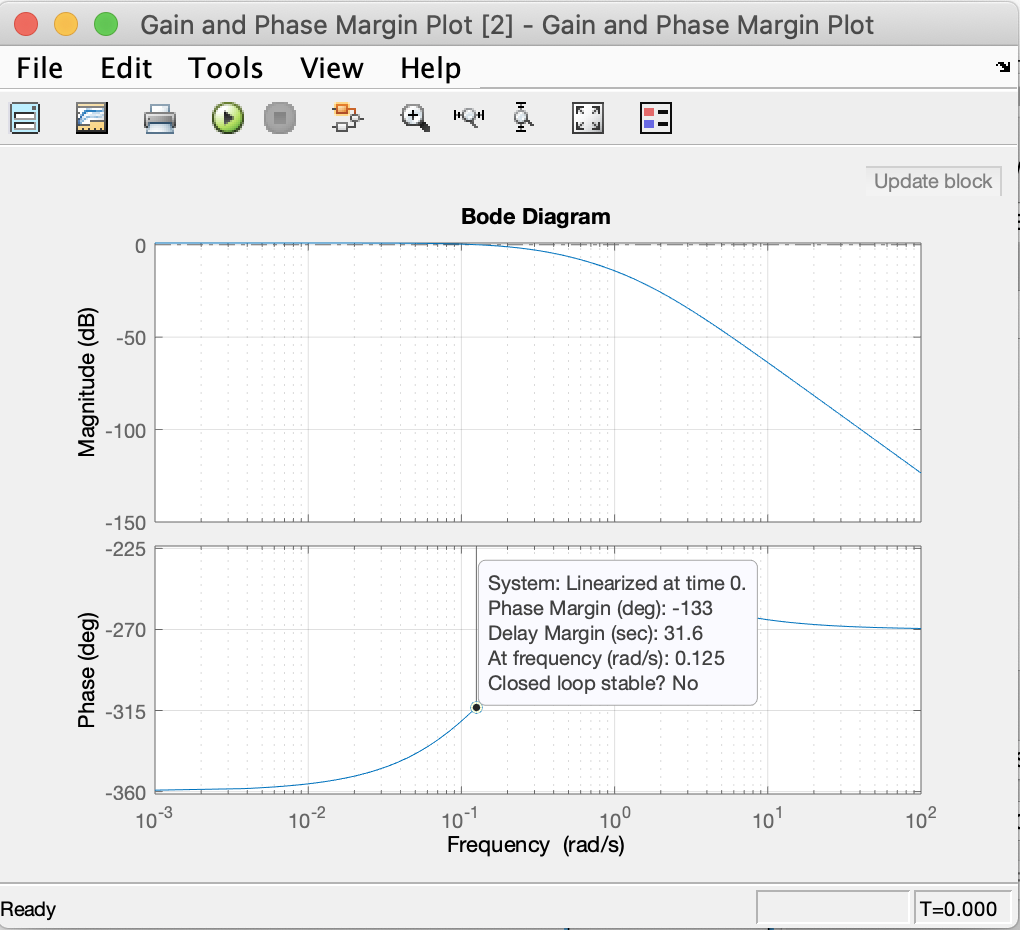
\includegraphics[width=12cm, height=10cm]{bode_plot.png}

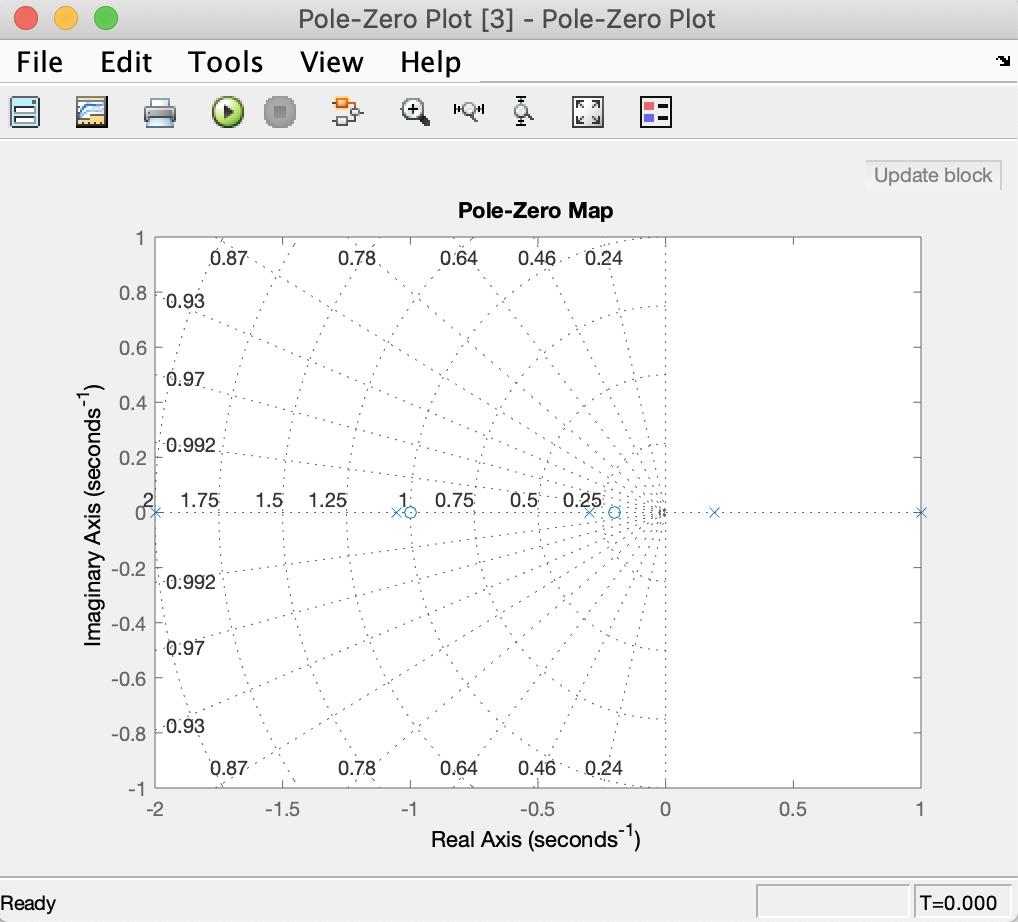
\includegraphics[width=12cm, height=10cm]{pole_zero_plot.png}

\begin{problem}
  \problemtitle{Part D}
  \problemquestion{Analyze Bode plot - calculate asymptotes and frequence breaks and put calculations in report. Also calculate intersections of the plot with axes.
}
  \problemsolution{
  Asymptotes were calculated by general function for calculating asymptotes https://lpsa.swarthmore.edu/Bode/BodeHowGen.htmlusing
  Computations were implemented by MATLAB functions (code is below)
  
  Frequence breaks are poles and zeros(roots of numerator and denominator) were calculated using MATLAB.
  
  
  
  }
\end{problem}


Roots of numerator
\begin{lstlisting}
>> roots(num)

ans =

  -0.6000 + 1.2806i
  -0.6000 - 1.2806i
\end{lstlisting}

Roots of denominator
\begin{lstlisting}
  >> roots(den)

ans =

  -2.0372 + 0.0000i
  -0.6175 + 0.6693i
  -0.6175 - 0.6693i
   0.9267 + 0.0000i
   0.1788 + 0.0000i
   
\end{lstlisting}

Frequency asymptotes pointwise graph generator
\begin{lstlisting}
function res = asymptotes_graph(w, n_roots, d_roots)
c_prime = 2/3 * prod(n_roots)/prod(d_roots);
first_term = 0;
s = size(n_roots);
first_vector = reshape(n_roots, 1, s(1));
for term = first_vector
    first_term = first_term + 20 * log10(abs(1 + 1i*w/term));
end

second_term = 0;
s = size(d_roots);
second_vector = reshape(d_roots, 1, s(1));
for term = second_vector
    second_term = second_term + 20 * log10(abs(1 + 1i*w/term));
end


res = 20 * log10(abs(c_prime)) + first_term - second_term;

\end{lstlisting}

intersections of the plot with axes
\begin{lstlisting}
>> asymptotes_graph(0, num_roots, den_roots)

ans =

   13.5556
   
>> asymptotes_graph(0.5733474, num_roots, den_roots)

ans =

    0.0273 (roundoff + plot error)
   
\end{lstlisting}

Bode plot with asymptotes with breakpoints in poles and zeros.

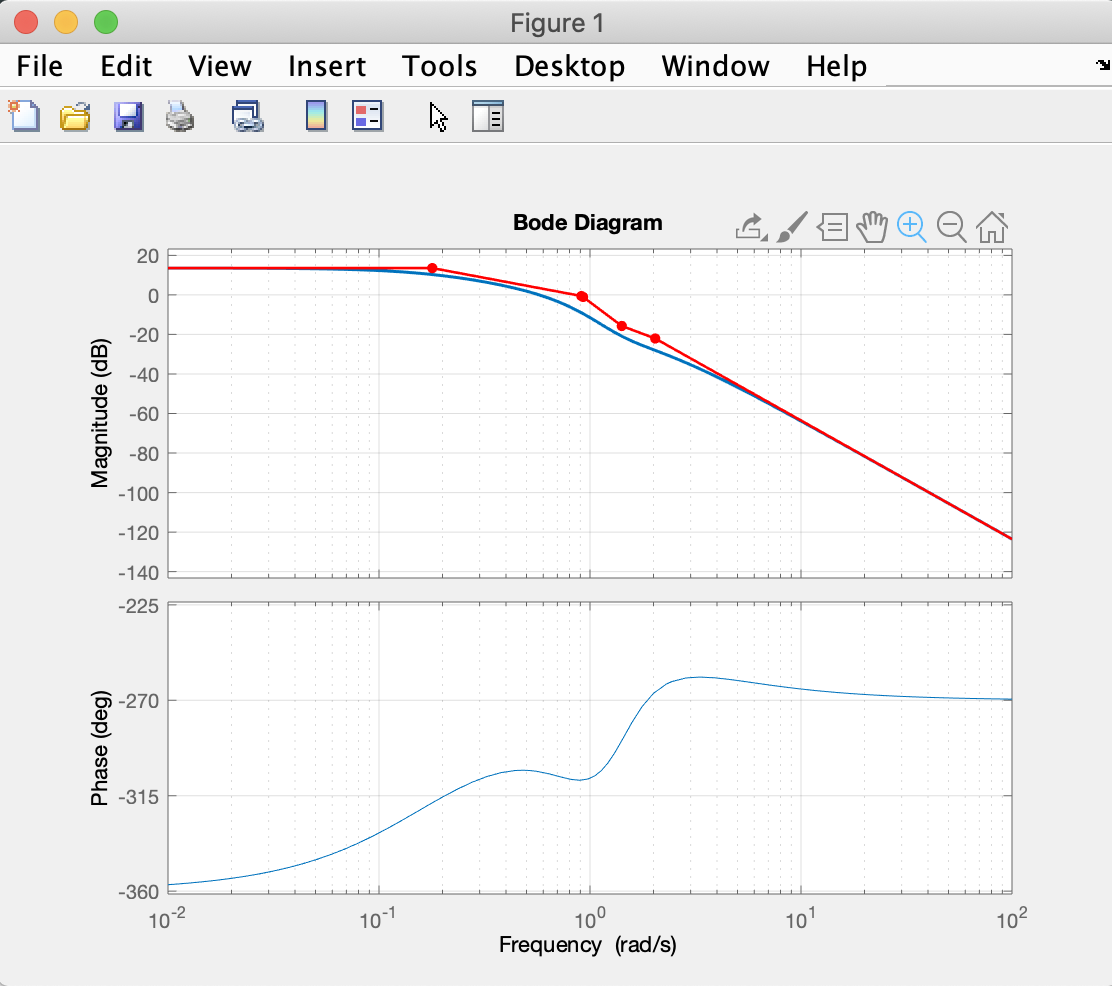
\includegraphics[width=14.3cm, height=10cm]{bode_plot_asymptotes.png}


\section*{Problem 2}

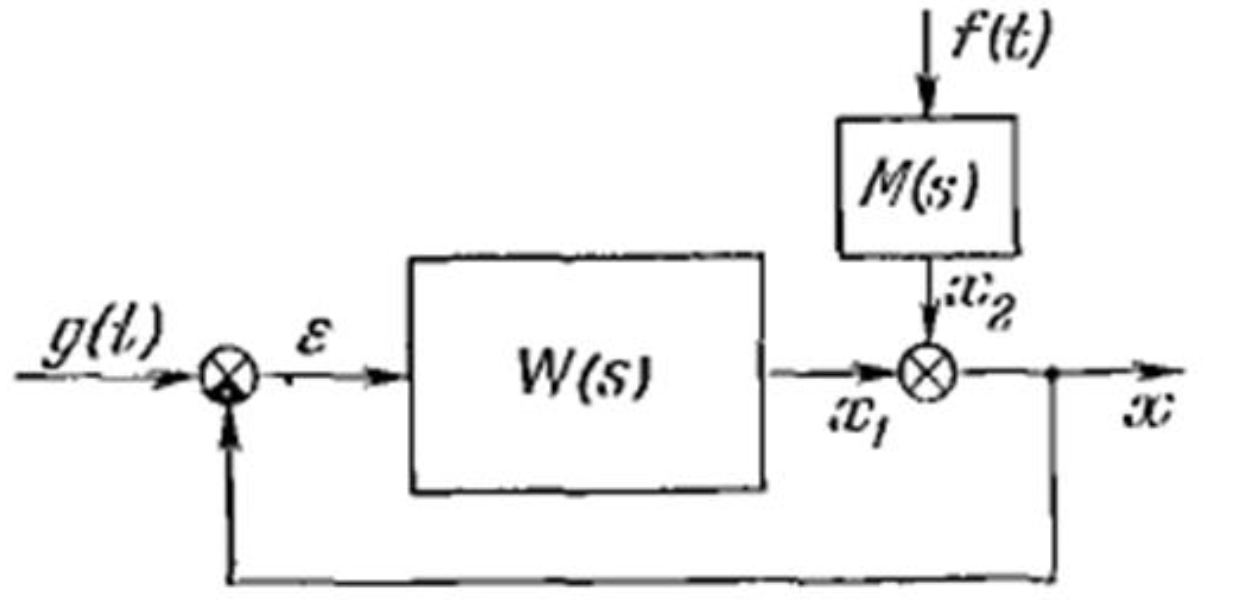
\includegraphics[width=15.3cm, height=8cm]{2.png}
$$W(s) = \frac{s+4}{3s+2}$$
$$M(s) = \frac{1}{s+1}$$
\begin{problem}
  \problemquestion{Find total transfer function for a closed-loop system.}
  \problemsolution{
      $$\Phi(s) = \frac{X}{G} = \frac{W(s)}{1 + W(s)}$$
      $$\Phi_f(s) = \frac{X}{F} = \frac{M(s)}{1 + W(s)}$$
      $$X = \Phi(s)G + \Phi_f(s)F = \frac{W(s)}{1 + W(s)}G + \frac{M(s)}{1 + W(s)}F$$
      $$X = \frac{\frac{s+4}{3s+2}}{1 + \frac{s+4}{3s+2}}G + \frac{\frac{1}{s+1}}{1 + \frac{s+4}{3s+2}}F$$
      $$X = \frac{s+4}{4s + 6}G + \frac{3s+2}{ (4s+6)(s+1)}F$$
      $$Answer: X = \frac{s+4}{4s + 6}G + \frac{3s+2}{4s^2 + 10s + 6}F$$
  }
\end{problem}

\section*{Problem 3}
$$A = \begin{pmatrix}
2 & 0\\ 
-3 & 1 
\end{pmatrix}, B = \begin{pmatrix}
-1\\ 
1 
\end{pmatrix}, C = \begin{pmatrix}
-2 & 0
\end{pmatrix}, D = \begin{pmatrix}
2
\end{pmatrix}$$
\begin{problem}
  \problemquestion{Find transfer function of the system.}
  \problemsolution{
    Using formula for converting SS to TF:
    $$Y(s) = \{C(sI - A)^{-1}B + D\}U(s)$$
    $$(sI - A) = \begin{pmatrix}
s - 2 & 0 \\
3 & s - 1
\end{pmatrix}$$
    $$(sI - A)^{-1} = \frac{1}{s^2-3s+2}\begin{pmatrix}
s - 1 & 0 \\
-3 & s - 2
\end{pmatrix}$$
$$C(sI - A)^{-1} = \frac{1}{s^2-3s+2}\begin{pmatrix}
2 - 2s & 0 \\
\end{pmatrix}$$
$$C(sI - A)^{-1}B = \begin{pmatrix}
\frac{2s - 2}{s^2-3s+2} \\
\end{pmatrix}$$
$$C(sI - A)^{-1}B + D = \begin{pmatrix}
\frac{2s^2-4s+2}{s^2-3s+2} \\
\end{pmatrix}$$
$$Answer: TF: \frac{2s^2-4s+2}{s^2-3s+2}$$
  }
\end{problem}

Answer validation in MATLAB
\begin{lstlisting}
>> A = [2 0; -3 1];
>> B = [-1;1];
>> C = [-2, 0];
>> D = [2];
>> [b, a] = ss2tf(A, B, C, D)
b = 2    -4     2
a = 1    -3     2
\end{lstlisting}



\section*{Problem 4}
$$A = \begin{pmatrix}
4 & 1\\ 
-2 & 1 
\end{pmatrix}, B = \begin{pmatrix}
2 & 1\\ 
3 & 0
\end{pmatrix}, C = \begin{pmatrix}
1 & 3
\end{pmatrix}, D = \begin{pmatrix}
1 & 2
\end{pmatrix}$$
\begin{problem}
  \problemquestion{Find transfer functions of the system.}
  \problemsolution{
      Using formula for converting SS to TF:
    $$Y(s) = \{C(sI - A)^{-1}B + D\}U(s)$$
    $$(sI - A) = \begin{pmatrix}
s - 4 & -1 \\
2 & s - 1
\end{pmatrix}$$
    $$(sI - A)^{-1} = \frac{1}{s^2-5s+6}\begin{pmatrix}
s - 1 & 1 \\
-2 & s - 4
\end{pmatrix}$$
$$C(sI - A)^{-1} = \frac{1}{s^2-5s+6}\begin{pmatrix}
s - 7 & 3s - 11 \\
\end{pmatrix}$$
$$C(sI - A)^{-1}B = \begin{pmatrix}
\frac{11s - 47}{s^2-5s+6} & \frac{s-7}{s^2-5s+6}\\
\end{pmatrix}$$
$$C(sI - A)^{-1}B + D = \begin{pmatrix}
\frac{s^2 + 6s - 41}{s^2-5s+6} & \frac{2s^2-9s+5} {s^2-5s+6} \\
\end{pmatrix}$$
$$Answer:
TF_1: \frac{s^2 + 6s - 41}{s^2-5s+6}, \hspace{0.5cm}
TF_2:\frac{2s^2-9s+5} {s^2-5s+6}$$
  }
\end{problem}


Answer validation in MATLAB
\begin{lstlisting}
>> A = [4 1; -2 1];
>> B = [2;3];
>> C = [1 3];
>> D = [1];
>> [b, a] = ss2tf(A, B, C, D)
b = 1.0000    6.0000  -41.0000
a = 1    -5     6


>> A = [4 1; -2 1];
>> B = [1;0];
>> C = [1 3];
>> D = [2];
>> [b, a] = ss2tf(A, B, C, D)
b = 2    -9     5
a = 1    -5     6
\end{lstlisting}


\section*{Problem 5}
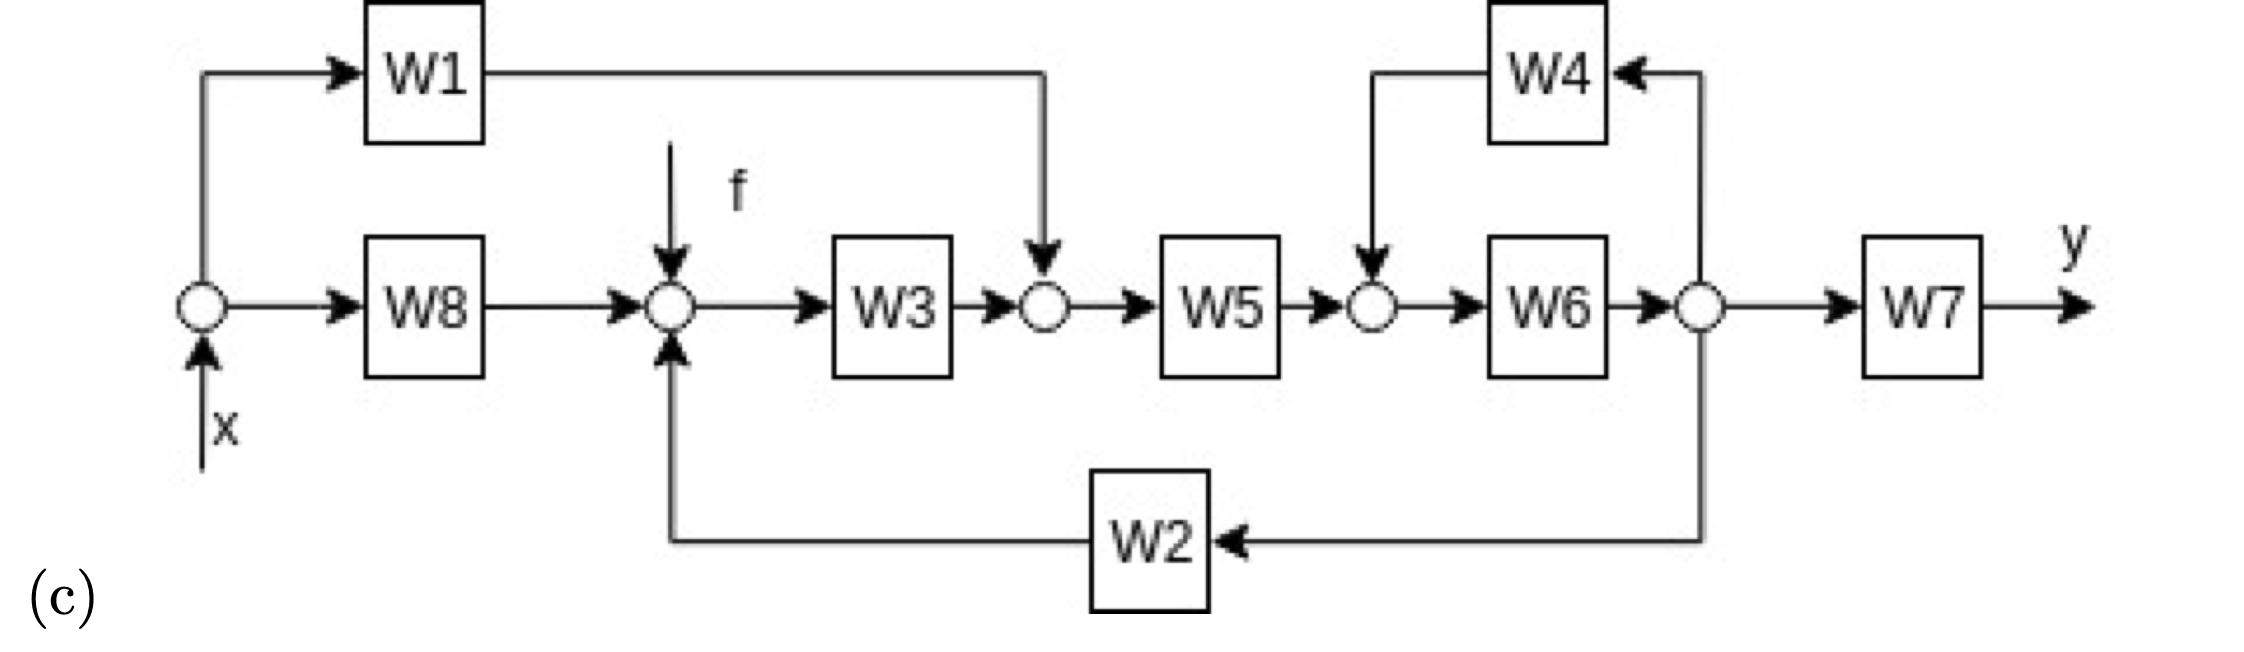
\includegraphics[width=15.3cm, height=5cm]{8.png}


\begin{problem}
  \problemquestion{Find the total transfer function of the system.}
  \problemsolution{
  $$\Phi(s) = \frac{Y}{X} = (W_8 + \frac{W_1}{W_3}) * \frac{W_3W_5W_6W_7}{1-W_6W_4-W_2W_5W_6}$$
  $$\Phi_f(s) = \frac{Y}{F} = \frac{W_3W_5W_6W_7}{1-W_6W_4-W_2W_5W_6}$$
  $$Y = \Phi(s)X + \Phi_f(s)F = \frac{W_3W_5W_6W_7}{1-W_6W_4-W_2W_5W_6} * ((W_8 + \frac{W_1}{W_3})X + F)$$
  
  $$Answer: Y = \frac{W_3W_5W_6W_7}{1-W_6W_4-W_2W_5W_6} * ((W_8 + \frac{W_1}{W_3})X + F)$$
  Reduction of Transfer function diagram is on the next page.
  }
\end{problem}
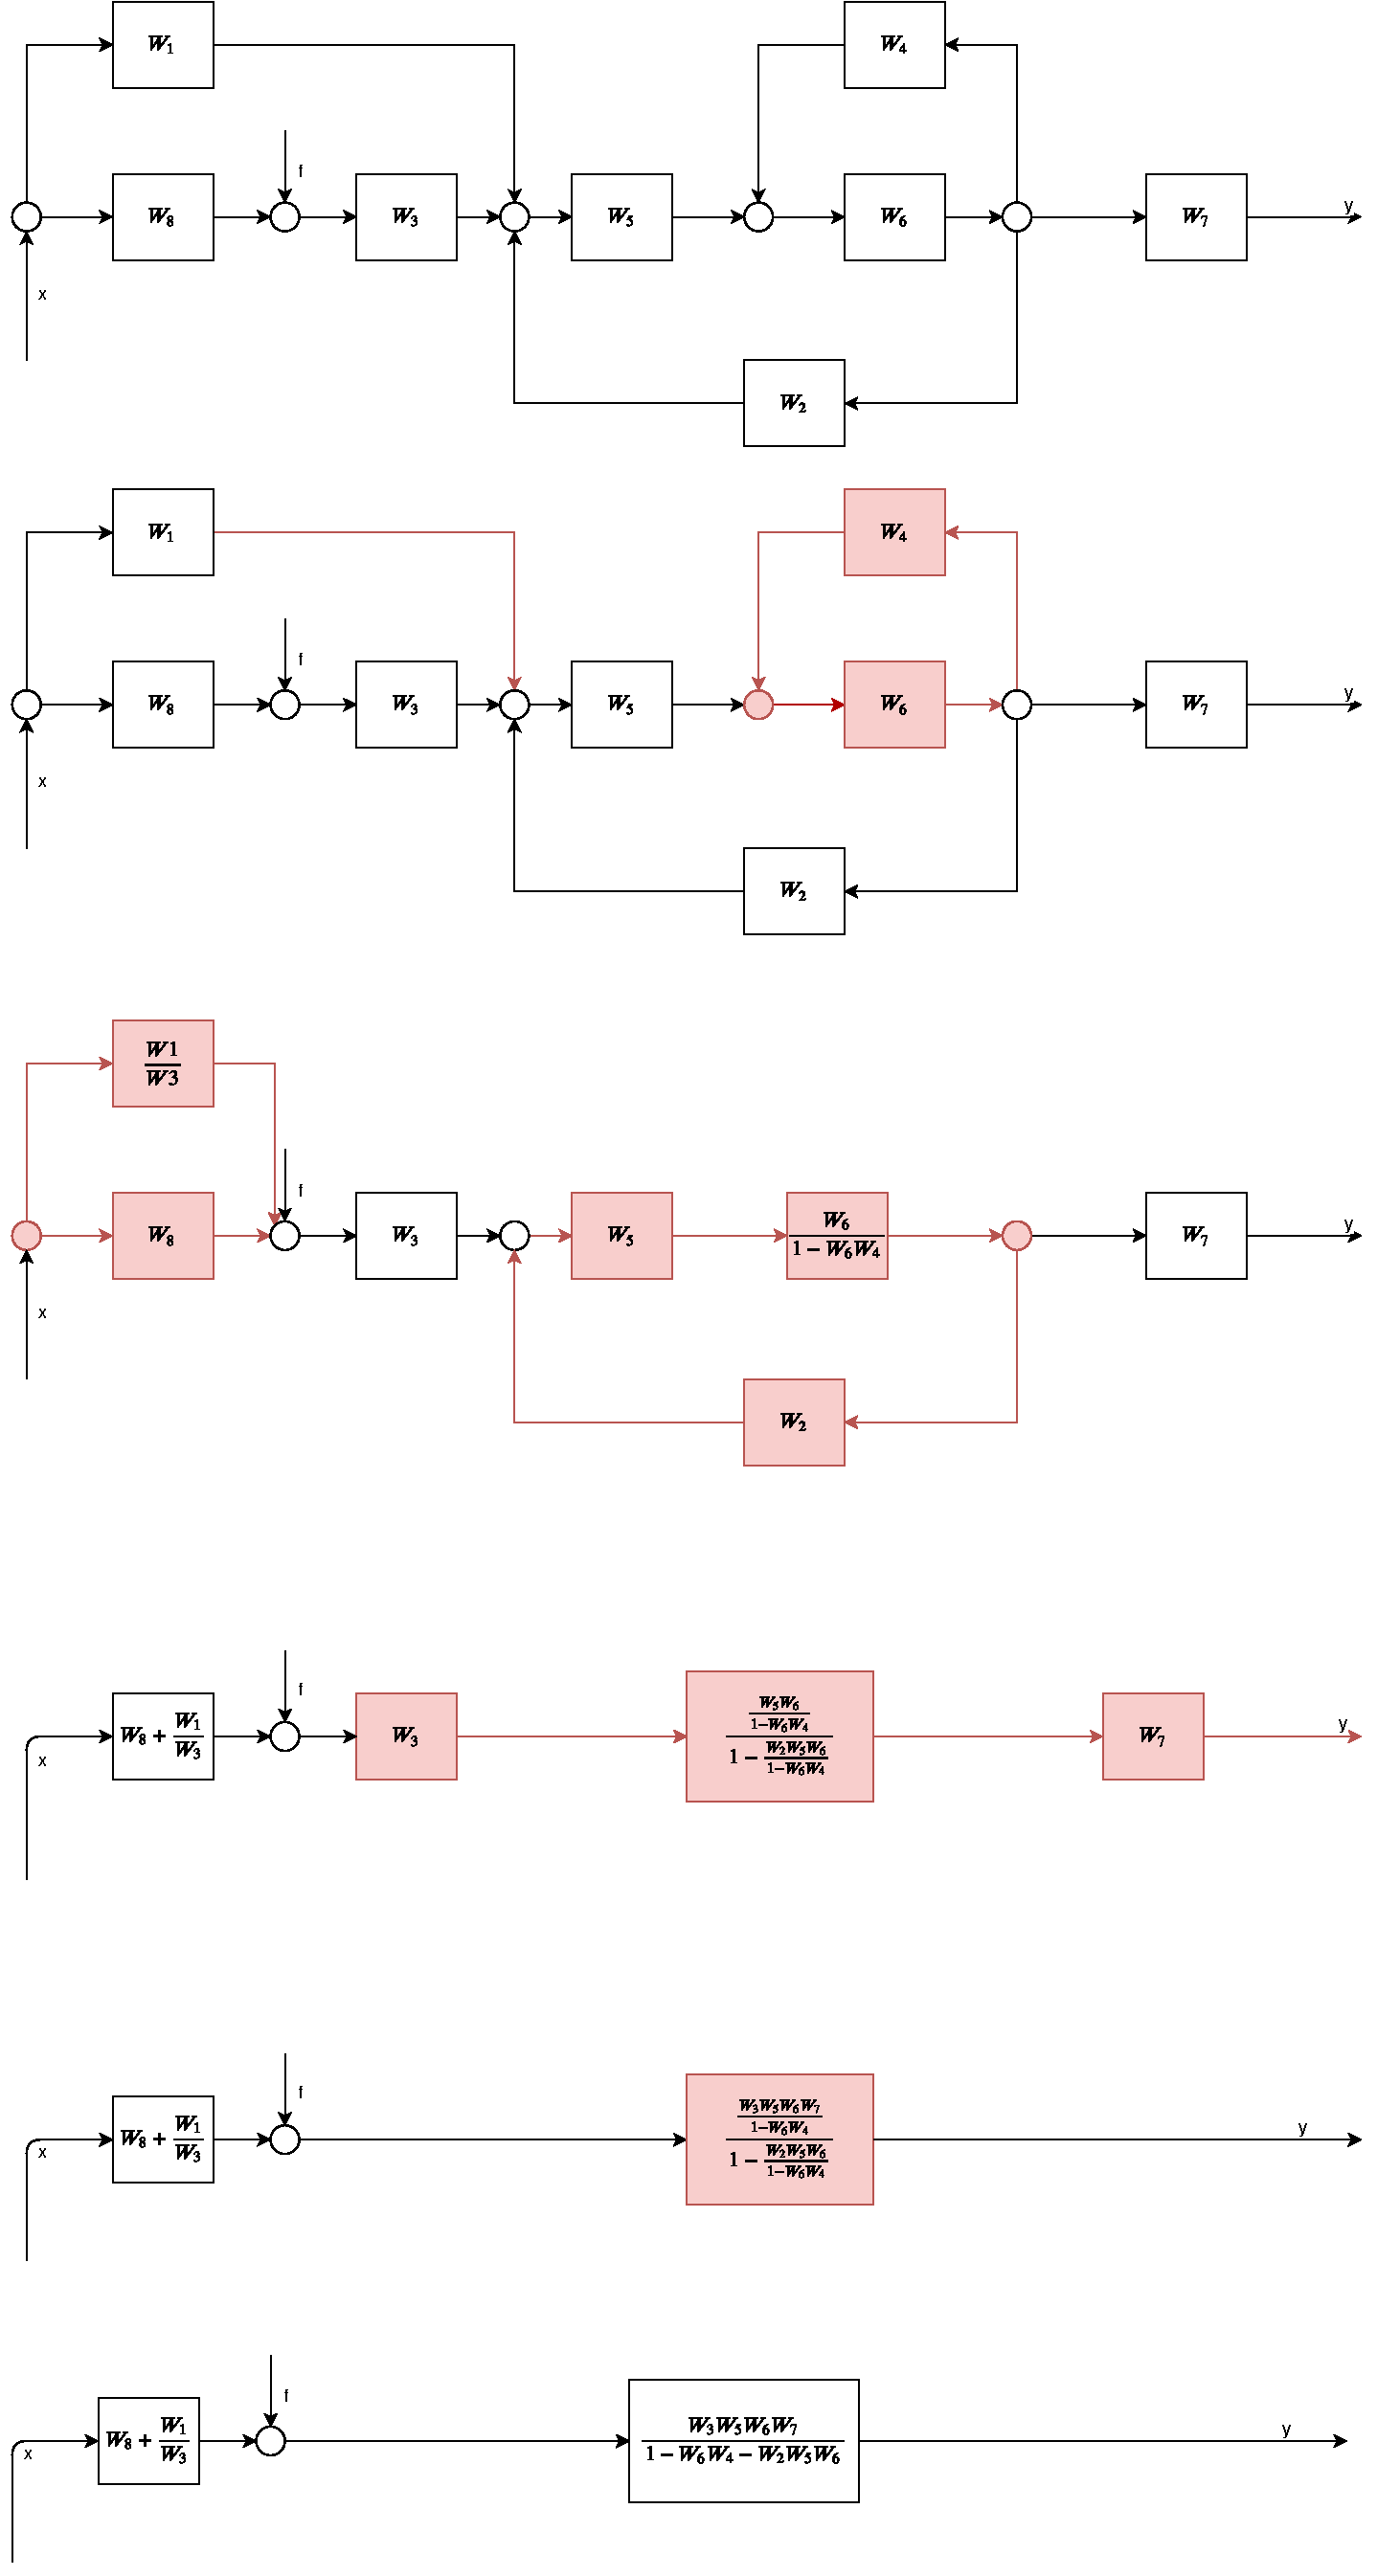
\includepdf[pages=-]{A5.pdf}




\end{document}
